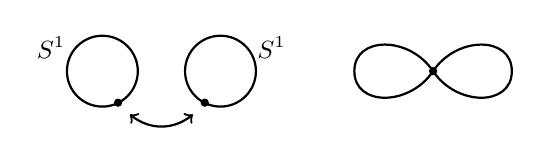
\begin{tikzpicture}[line width=0.8pt, every node/.style={font=\small}]
  \draw (0,0.45) circle (0.45);
  \fill (0.2,0.05) circle (1.5pt);
  \node at (-0.65,0.75) {$S^1$};
  \draw (1.5,0.45) circle (0.45);
  \fill (1.3,0.05) circle (1.5pt);
  \node at (2.15,0.75) {$S^1$};
  \draw[<->] (0.35,-0.1) .. controls (0.6,-0.3) and (0.9,-0.3) .. (1.15,-0.1);
  \node at (2.75,0.45) {$\rightsquigarrow$};
  \begin{scope}[shift={(4.2,0.45)}]
    \draw (0,0) .. controls (-0.3,0.45) and (-1.0,0.45) .. (-1.0,0) .. controls (-1.0,-0.45) and (-0.3,-0.45) .. (0,0);
    \draw (0,0) .. controls (0.3,0.45) and (1.0,0.45) .. (1.0,0) .. controls (1.0,-0.45) and (0.3,-0.45) .. (0,0);
    \fill (0,0) circle (1.5pt);
  \end{scope}
\end{tikzpicture}
